\documentclass[12pt]{article}
\usepackage[utf8]{inputenc}
\usepackage[spanish]{babel}
\usepackage{graphicx}

\usepackage[a4paper, top=2cm, bottom=2cm, left=2.5cm, right=2.5cm]{geometry}

\usepackage[breaklinks]{hyperref}

\setlength{\parskip}{.8em}
\renewcommand{\baselinestretch}{1.15}

\title{Proyecto SNAKE}
\author{Barreiro Valdez Alejandro\\Piña Félix Emilio\\Zepeda Baeza Jessica}
\date{18 de diciembre de 2021}

\begin{document}

\begin{center}
    
\includegraphics[width = 4cm]{img/logo/unam-escudo-azul.png}
    \hspace{7cm}
    
\includegraphics[width = 4cm]{img/logo/fi.jpg}
    \vspace{4cm}
    
    \huge
    \textbf{Proyecto SNAKE}
    \vspace{.5cm}
    
    \LARGE
    Barreiro Valdez Alejandro\\Piña Félix Emilio\\Zepeda Baeza Jessica
    
    \noindent\rule{10cm}{0.4pt}
    \vspace{4cm}
    
    \large
    18 de diciembre de 2021
    \vspace{1cm}
    
    \textsc{\Large Estructura y Programación de Computadoras}
    \vspace{.5cm}
    
    \flushleft
    \textbf{Grupo:} 2
    
    \textbf{Profesor:} Luis Sergio Durán
\end{center}

\newpage

\section*{Introducción}

\subsection*{Descripción}
En este proyecto se realizó un juego \textit{Snake} utilizando lenguaje ensamblador. El juego utiliza las funcionalidades básicas de este juego clásico y genera una interfaz gráfica donde se puede jugar. El programa cuenta con \textit{scores} que le permiten saber su rendimiento al usuario. Además, se tiene una velocidad para que el jugador se ponga a prueba con velocidades altas o practique bajando la velocidad. El juego desarrollado también cuenta con diferentes estados: estado de pausa, estado \textit{play} para jugar una partida y estado de reinicio para terminar una partida y reiniciar los datos. El juego capta datos de entrada del teclado y del mouse para que el usuario pueda manipular el juego. Se utilizan las teclas para mover la serpiente y el mouse para manipular los diferentes botones. Con todas estas funcionalidades se tiene un juego \textit{Snake} funcional listo para ser utilizado por un jugador.

\subsection*{Planteamiento del Problema}
El proyecto fue desarrollado a partir de un código base proporcionado por el profesor. El código base contiene, en su mayoría, código que genera una interfaz de usuario con la cual se debe generar el juego. Esta interfaz del usuario tiene dos partes, una donde se manipulan ciertos botones para el juego y otra donde se hace el juego de la serpiente. Se debe generar código para que ambas partes sean funcionales y haya movimientos en la interfaz de usuario. El código base también proporciona una estructura del programa principal donde se tiene un \textit{loop} que analiza el estado del mouse. En esta parte es donde se desarrolló la mayoría de los aportes hechos para que el juego funcione. Los problemas generales que surgieron al desarrollar este código consisten en modificar la interfaz gráfica para que haya movimiento y se sigan las reglas de este juego. Se deben coordinar los botones del juego y los \textit{scores} para generar una sesión de partida y que el usuario pueda correr dicho código como si fuera un juego más. Esto no es tarea fácil ya que el lenguaje en el que se realizó es en lenguaje ensamblador.


\section*{Desarrollo}

\subsection*{Planteamiento y justificación de la solución}
Antes de generar algún cambio sobre la lógica del juego se realizaron algunos cambios para facilitar la comprensión y codificación del código base. Lo primero que se generó fueron tres variables para almacenar los datos de la cabeza de la serpiente. En el código base se hacía uso de una sola variable donde se dividían los bits para darle un valor a cada variable. Se cambió esto para tener un manejo más fácil de las diferentes variables de la cabeza y no tener que estar obteniendo bits cada vez que se quiera manipular la cabeza. Se creó una variable para la columna, la fila y la dirección de la cabeza. También se modificó la manera en que se guarda el cuerpo de la serpiente. El primer elemento del arreglo es el más cercano a la cabeza y estos elementos solo contienen la fila y la columna de cada parte del cuerpo. En este caso sí se divide la parte alta y la parte baja de cada uno de los elementos, pero esto no implica muchas complicaciones ya que se puede realizar fácilmente la separación utilizando registros de la parte alta o baja. Para generar movimiento se recorren las posiciones del cuerpo, por lo que cada una contiene el valor de su antecesor. Por esto mismo es que no se necesita una variable de dirección para todos los elementos. También se completó el procedimiento para borrar al jugador. Se tomó la lógica de los procedimientos para dibujar la cabeza y el cuerpo y se utilizó para dibujar un carácter negro con fondo negro para eliminar el elemento. De esta manera se pinta de negro toda la serpiente. Estos fueron los cambios realizados en el código base antes de empezar a codificar funcionalidades como el movimiento y los botones.

\subsubsection*{Lógica de botones}
Lo primero que se realizó fue la lógica para que los botones sirvan. Esto se realizó identificando en qué renglones se presiona el click izquierdo después de convertirlo a la resolución deseada. El único botón que ya estaba programado era el de salir, a partir de éste se diseñaron los demás. Primero se checa en qué renglones se encuentra el click: si en los del botón de salir, si en los botones de velocidad o si en los botones de estado del juego. A partir de ahí se salta hacia el botón que se detectó y se verifica entre qué columnas se encuentra el click. Las columnas dan la información concreta sobre si se está presionando un botón o no. Si no se está presionando ningún botón se repite el proceso de leer el estado del mouse y si se está haciendo un click. Para los botones de velocidad se incrementa o decrementa el valor de \textit{speed} y se llama a imprimir la nueva velocidad. Para los botones de estado se cambia el estado del programa y se reinicia la posición de la serpiente si es necesario. Con esta lógica de botones se identifica dónde se genera un click izquierdo y se genera una acción dependiendo del botón.

\subsubsection*{Lógica del movimiento de la serpiente}
Posteriormente, se realizó el movimiento del jugador utilizando un procedimiento MOVER para mover la serpiente en una dirección cada determinada cantidad de tiempo. Para determinar la cantidad de tiempo que ha transcurrido en el programa se creó un procedimiento llamado CRONO donde se actualizan los milisegundos que han transcurrido en el programa. Este procedimiento utiliza los ticks del sistema y los convierte a milisegundos. La idea para mover la serpiente es que se mueva cada cantidad de tiempo dependiendo de la velocidad. Para probar esta funcionalidad se programó que la serpiente se moviera cada medio segundo y que cuando se terminara de mover leyera los ticks para reiniciar el tiempo transcurrido. El tiempo entre cada movimiento se calculó después utilizando los datos de \textit{speed}. 

Después, se codificó el movimiento de la serpiente utilizando la dirección de la cabeza. Primero, se borra al jugador para eliminar las posiciones anteriores. Se recupera el valor de la columna y del renglón de la serpiente para modificarlos y utilizarlo para asignaciones posteriores. Una serie de condicionales permitirán modificar el renglón o columna de la cabeza para que esta se mueva dependiendo de la dirección que se tiene. Ya modificada la cabeza, se modifican los valores del cuerpo. Estos valores se modifican recorriendo hacia la derecha todos los valores hasta que se encuentre un cero en el arreglo. Cuando se encuentra con un cero se deja de modificar el arreglo. De esta manera cada uno de los elementos del cuerpo se mueve hacia donde se encontraba la siguiente posición más cercana al cuerpo. Por último, se modifica el elemento que se encuentra más cercano al cuerpo para asignarle el valor anterior de la cabeza y se imprime el jugador. En este procedimiento también se realiza la validación que no se haya comido ningún marco del juego. Esta parte del juego se codificó después de la lógica de teclas para indicar la dirección del movimiento ya que anterior a esto solo se tenía una serpiente que se movía en una dirección que se debía indicar en el código. Por lo mismo se explicará después de la lógica de teclas.

\subsubsection*{Lógica de lectura de teclas}
El siguiente paso en la creación del juego fue la codificación de la lectura de teclas y el cambio de dirección. Esta parte se hizo antes de la conversión de la resolución del mouse. Se utilizó una interrupción para detectar si hay contenido en el \textit{buffer} del teclado y si hay algo se lee dicha tecla. Si no existe nada en el \textit{buffer} se continúa la ejecución. Si el programa acaba de pasar por el estado de STOP entonces la dirección se cambia a que sea la derecha forzosamente. De otra manera, primero se valida hacia qué lado se puede mover la serpiente. Si la serpiente tiene un movimiento vertical, su siguiente movimiento solo puede ser horizontal y viceversa. Sabiendo las teclas que sí pueden afectar el valor de la dirección, se compara el valor ASCII de la tecla leída con los de A, S, D o W y si en alguna coinciden los valores se cambia la dirección de la cabeza. De otra manera, no se realiza ningún cambio de dirección. Para la siguiente iteración, la dirección de la serpiente habrá cambiado y esto se verá reflejado gracias al procedimiento para mover la serpiente. Lo siguiente que se modificó fue el cálculo de la velocidad para que la serpiente se pueda mover más rápido o más lento dependiendo de lo que indique el usuario.

\subsubsection*{Cálculo de velocidad}
Para el cálculo de la velocidad a la que se mueve la serpiente se creó un procedimiento llamado CALCULO\_SPEED donde se utiliza el valor de la velocidad y un indicador que proporciona un valor para cada cuánto tiempo se debe mover la serpiente. El tiempo máximo e inicial entre cada movimiento es de 300 milisegundos, este tiempo disminuye por 3 milisegundos por cada que la velocidad aumenta en uno por lo que el tiempo mínimo entre movimientos es de 3 milisegundos. El rango de la velocidad se encuentra entre 0 y 99. El procedimiento mencionado realiza una resta de los 300 milisegundos con el valor de la velocidad por tres para obtener un indicador de cada cuántos milisegundos se debe mover la serpiente. Dicho indicador es utilizado junto con los milisegundos transcurridos para mandar a llamar el procedimiento que mueve la serpiente. La velocidad solo puede aumentar al iniciar el juego, después de un reinicio del juego y cuando se come un objeto. Cuando se come un objeto la velocidad aumenta en dos. El cálculo del indicador de la velocidad se realiza antes de la comparación con los milisegundos transcurridos y de la llamada al procedimiento de mover si es que este es necesario. El cálculo de la velocidad se realizó como una resta para que el cambio entre cada intervalo fuera uniforme. Además, se realizó una bandera para saber cuándo se puede modificar la velocidad utilizando los botones. Esta bandera es activada cuando se pasa al estado de reinicio y se desactiva cuando se pasa a \textit{play}. Lo siguiente que se codificó fue la lógica de cómo comer uno de los objetos verdes.

\subsubsection*{Lógica del objeto a comer}
Una vez que la serpiente fue capaz de desplazarse por el área de juego se realizó el procedimiento CALCULO\_ITEM. Este procedimiento calcula un número aleatoriamente tanto para el renglón como para la columna y los guarda en dos variables en memoria. La forma de obtener el número aleatorio es leyendo los ticks del sistema y dividiendo la parte baja (que varía más) entre un número n. Al tomar el residuo de esta división se obtiene un rango de valores de 0 a n-1. Después se suma una constante al número obtenido y así se obliga que número se encuentre entre un rango de valores. Por ejemplo, en el caso de las columnas se dividió sobre 58 y se sumó 21 para obtener un número entre 21 y 78. Al final, el procedimiento compara las coordenadas obtenidas con la cabeza y cuerpo de la serpiente; de manera que si son iguales, se calculan nuevas coordenadas. 

\subsubsection*{Acción de comer}
El comer un objeto es el objetivo principal del juego; por lo tanto, se realizó un procedimiento especial para realizar esta acción. El procedimiento COMER\_OBJ funciona de una manera bastante sencilla. Primero, se guardan los valores de columna y renglón del objeto. Después se compara con el valor que tiene la cabeza de la serpiente. En caso de que sean iguales se va a entrar en una serie de instrucciones que solo aplican para este caso. Lo primero que sucede después de la comparación es la llamada al procedimiento CALCULO\_ITEM seguido por el procedimiento que se encarga de imprimir el objeto verde. Después, se utiliza el contador de la cola para usarlo como índice. Se iguala la nueva posición de la cola a un valor diferente de cero. Como el valor nuevo es diferente de cero, el procedimiento que imprime a la serpiente va a imprimir un nuevo bloque que corresponde a la nueva cola. Se incrementa el contador de la cola. Como al comer un objeto se considera que se sube el nivel, se incrementa la velocidad del juego en 2 cada vez que se come un objeto. Cada objeto que se come equivale a 10 puntos en el juego, por lo que se incrementa el valor del score. Se llama al procedimiento IMPRIME\_SCORE para que se vaya actualizando el valor que se ve en pantalla. También se hace una comparación del \textit{score} con el \textit{high-score}, ya que si se supera el último, éste se tiene que actualizar. Si se actualiza, también se imprime en pantalla. Si no son iguales, se termina el procedimiento y sigue la ejecución del programa. Este procedimiento se llama cada vez que se mueve la serpiente, ya que se necesita comparar si se ha comido un objeto en cada posición que adquiere la cabeza de la serpiente. Esto se hace dentro del procedimiento MOVER, una vez que se hayan actualizado los valores de posición.  

\subsubsection*{Estado Stop y reinicio}
Hasta este punto existen dos estados en el juego: pausa (representado en código con 0 y donde la serpiente se detiene en un punto específico) y \textit{play} (representado en código con 1 y donde el juego está activo). Por lo que lo siguiente a crear es el estado \textit{Stop} (representado en código con 2) el cual se activa cuando el botón Stop es presionado y cuando el juego termina, ya sea porque la serpiente chocó con un marco o consigo misma. Se creó un procedimiento llamado STOP que básicamente detiene a la serpiente, hace que parpadee dos veces, restablece los datos necesarios iniciales mediante otro procedimiento llamado REGRESA\_DATOSIN e imprime dichos datos. El parpadeo se realiza borrando e imprimiendo la serpiente dos veces gracias a un ciclo que espera hasta que hayan pasado cinco ticks, esto comparando un tick inicial cuando se modifica a la serpiente con uno dentro del ciclo. Se hace uso de un contador que es par cuando se necesita borrar la serpiente e impar cuando se necesita imprimir; de esa forma se sabe a que flujo dirigirse. 

Después del parpadeo se borra la serpiente y se llama al procedimiento REGRESA\_DATOSIN. En este procedimiento se cambia el valor de la cabeza al inicial. Después se borra toda la cola utilizando la variable \textit{tail\_conta} para realizar un ciclo que vuelve cero a todos los elementos de la cola y otro ciclo donde se restablecen los cuatro elementos iniciales. Se modifica la variable anterior así como aquellas concernientes a \textit{score}, \textit{speed}, la dirección en la que se mueve la serpiente, el estado se vuelve 0 (pausa) y se activa una bandera llamada \textit{banStop} que indicará en el flujo principal que se acaba de pasar por el procedimiento STOP. De esa manera, al presionar \textit{Play} y continuar con el juego se verificará si esa bandera está activa (toma un valor de 1) y si es así, no se leerá la tecla en el \textit{buffer} para forzar que se mueva a la derecha y se desactivará la bandera \textit{banStop}. Otras modificaciones en el flujo principal son que al presionar el botón de \textit{stop}, cambia la variable del \textit{status} a 2. Además, se incluye una comparación después de verificar si el estado es pausa y antes de iniciar todo el movimiento de la serpiente donde se verifica si el estado es \textit{stop}. En caso de que lo sea, se llama al procedimiento STOP y una vez realizado, se sigue el flujo como si estuviera en pausa. 

\subsubsection*{Comer marcos}
Como se sabe, en el juego de \textit{Snake} no se puede tocar los marcos del juego. De ser así, se acaba el juego. Para que en nuestra versión del juego se muestre este funcionamiento de la misma manera se creó un procedimiento llamado COMER\_MARCO. Este procedimiento compara el valor del renglón de la cabeza (para los marcos inferior y superior), y el valor de la columna de la cabeza (para los marcos izquierdo y derecho). Este procedimiento también se llama dentro del procedimiento MOVER. Para que no se imprima la serpiente en el caso de que si haya tocado un marco, este procedimiento se llama después de haber actualizado los valores de la cabeza, pero sin haber impreso el cuerpo en pantalla. Un problema que se tenía cuando se llamaba al procedimiento STOP después de que se tocaba un marco es que se eliminaba el carácter del marco en el que se posaban los valores de la cabeza. Este problema se resolvió decrementando o aumentando (según el marco que se toque) el valor de la cabeza de la serpiente, regresando los valores a la posición inmediata previa a el toque del marco. Esto actúa análogamente a un cuello de tortuga. De esta manera al llamar al procedimiento STOP, en el que se borra a la serpiente, se borra únicamente su cuerpo dejando a los marco intactos. 

\subsubsection*{Que no se coma a sí misma}
Lo último que se realizó fue la funcionalidad para que la serpiente no se coma a sí misma. Para cuando se codificó esto ya se tenía un procedimiento para cuando la serpiente intenta comerse un marco por lo que ya se sabía cómo reiniciar la serpiente cuando ésta pierde. El problema en este caso fue cómo verificar que se ha perdido porque la serpiente se come a sí misma. Para esto se generó un procedimiento donde se compara cada una de las posiciones de la serpiente con la cabeza y si se coincide en columna y en renglón esto significa que la cabeza se encuentra en la misma posición que algún elemento del cuerpo. Cuando esto ocurre, la serpiente se está comiendo a sí misma por lo que se cambia el estado del programa para que se reinicie el juego. Si no coincide ninguna posición, el movimiento y el estado permanece de manera normal. Se realizó este proceso dentro de mover para que la serpiente sí se coma y se muestre la animación del parpadeo pero con la serpiente comiéndose a sí misma. Este fue el último gran cambio al proyecto y con este se completaron las diferentes funcionalidades que se requerían para generar un juego funcional de \textit{Snake}.

\subsection*{Diagrama de flujo y pruebas de escritorio}
\subsubsection*{Flujo principal}
En el Diagrama \ref{fig:main} se describe el flujo principal del programa. En él se analizan los botones y teclas presionadas de manera que se puede saber hacia donde mover la serpiente, el estado del juego (activo, inicial, terminado y en pausa), cuándo mover la serpiente y todo lo que esto implica. Las pruebas de escritorio abarcan algunas de las transiciones entre estados que pueden existir en el juego como Inicial - Activo, Activo - Inicial y Activo - Terminado. Ya que en en algún momento del diagrama se necesitan los datos que modifica algún procedimiento se tomarán valores arbitrarios para dichas variables. La primera prueba seguirá el flujo cuando no se encuentra el driver del mouse. La segunda prueba probará regresar en la dirección contraria en la venía la serpiente, presionar una tecla que no es A, S, D o W e intentar modificar la velocidad en estado Activo. 

\begin{enumerate}
    \item Prueba 1:
    \begin{itemize}
    \item DS = ES = @data (Se incializan registros)
    \item comprueba\_mouse \\ AX = 0000h (No se encuentra driver del mouse)
    \item ¿AX == FFFFh? FALSE
    \item DX = Dirección de la cadena no\_mouse
    \item AX = 0900h \\ int 21h (se imprime la cadena)
    \item AH = 08 \\ int 21h (se lee un caracter) \\AL = 35h (suponiendo que el usuario ingresa un 5)
    \item ¿AL == 0D? FALSE
    \item AH = 08 \\ int 21h (se lee un caracter) \\AL = 0Dh (suponiendo que el usuario ingresa un Enter)
    \item ¿AL == 0D? TRUE
    \item clear (macro que limpia pantalla) \\ AX = 4C00h \\int 21h (se pasa el control al sistema operativo)
    \item Fin del programa
\end{itemize}
    \item Prueba 2:
    \begin{itemize}
        \item DS = ES = @data (se incializan registros)
        \item comprueba\_mouse \\ AX = FFFFh (se encuentra driver del mouse)
        \item ¿AX == FFFFh? TRUE
        \item clear (se limpia la pantalla) \\ oculta\_cursor\_teclado \\ apaga\_cursor\_parpadeo \\ call DIBUJA\_UI (se dibuja la interfaz)
        \item delimitar\_cursor \\ muestra\_cursor\_mouse \\ posiciona\_cursor\_mouse
        \item leer\_ticks \\ t\_inicial == 0000 00001h 
        \item lee\_mouse \\ BX = 0000h (suponiendo que el botón izquierdo no está presionado)
        \item ¿BX == 0001? FALSE 
        \item lee\_mouse \\ BX = 0001h (suponiendo que el botón izquierdo está presionado)
        \item ¿BX == 0001? TRUE
        \item ¿status == 0? TRUE (el estado inicial es pausa y la serpiente no se mueve)
        \item lee\_mouse (suponiendo que se acaba de dar clic en el botón play) \\ BX = 0001h\\ CX = 80h \\ DX = A8h (valores que regresa la interrupción)
        \item AX = DX = A8h \\ AL = A8h/8 = 21d = 15h \\ AH = A8\%8 = 0 \\ AH = 0 \\DX = 15h (se obtiene el renglón en resolución correcta)
        \item AX = CX = 80h \\ AL = 80h/8 = 16d = 10h \\ AH = 80h\%8 = 0 \\ AH = 0 \\CX = 10h (se obtiene la columna en resolución correcta)
        \item ¿BX = 0001h? TRUE (se presionó el botón izquierdo)
        \item Se realiza la lógica de botones para identificar que se presionó Play \\ status = 1
        \item lee\_mouse \\ BX = 0001h
        \item ¿BX = 0001h? TRUE
        \item ¿status == 0? FALSE
        \item ¿status == 2? FALSE
        \item call CALCULO\_SPEED \\ speed\_indicator = 0 (valor que regresa el procedimiento)
        \item AX = speed\_indicator = 0
        \item ¿milisegundos $\leq$ AX? TRUE
        \item call CRONO (se actualiza el valor de milisegundos) \\ milisegundos = 0005h
        %\leq less or equal, \geq great or equal
        \item AH = 01h \\ int 16h (se lee el estado del buffer) \\ Z = 1 (la interrupción activa la bandera Z)
        \item ¿Z == 1? TRUE (no hay contenido en el buffer)
        \item lee\_mouse (suponiendo que no se dio clic) \\ BX = 0000h\\ CX =  \\ DX = 0 (valores que regresa la interrupción)
        \item AX = DX = 0 \\ AL = 0/8 = 0 \\ AH = 0\%8 = 0 \\ AH = 0 \\DX = 0 (se obtiene el renglón en resolución correcta)
        \item AX = CX = 0 \\ AL = 0/8 = 0 \\ AH = 0\%8 = 0 \\ AH = 0 \\CX = 0 (se obtiene la columna en resolución correcta)
        \item ¿BX = 0001h? FALSE 
        \item ¿status == 0? FALSE
        \item ¿status == 2? FALSE
        \item call CALCULO\_SPEED \\ speed\_indicator = 0 (valor que regresa el procedimiento)
        \item AX = speed\_indicator = 0
        \item ¿milisegundos $\leq$ AX? FALSE
        \item call MOVER (se mueve un espacio a la derecha la serpiente)
        \item call CRONO (se actualiza el valor de milisegundos) \\ milisegundos = 0007h
        \item AH = 01h \\ int 16h (se lee el estado del buffer) \\ Z = 0 (la interrupción no activa la bandera Z)
        \item ¿Z == 1? FALSE (hay contenido en el buffer, suponiendo que se oprimió la tecla A)
        \item ¿banStop == 1? FALSE (no se ha pasado por el procedimiento STOP)
        \item AH = 00h \\ int 16h (se lee el buffer) \\ DL = 97d (la interrupción regresa el ASCII de la tecla presionada en DL)
        \item ¿head\_dir == 0? TRUE
        \item ¿AL == 119d? FALSE
        \item ¿AL == 115d? FALSE (no puede regresar en la dirección en la que venía entonces no se modifica head\_dir) 
        \item lee\_mouse \\ BX = 0001h\\ CX = 88h \\ DX = 68h (valores que regresa la interrupción)
        \item AX = DX = 68h \\ AL = 68h/8 = 13d = 0Dh \\ AH = 68h\%8 = 0 \\ AH = 0 \\DX = 0Dh (se obtiene el renglón en resolución correcta)
        \item AX = CX = 88h \\ AL = 88h/8 = 17d = 11h \\ AH = 88h\%8 = 0 \\ AH = 0 \\CX = 11h (se obtiene la columna en resolución correcta)
        \item ¿BX = 0001h? TRUE
        \item Se realiza la lógica de botones para identificar que se presionó Speed Up, como se encuentra en estado activo o Play, no se modifica nada
        \item lee\_mouse \\ BX = 0001h
        \item ¿BX = 0001h? TRUE
        \item ¿status == 0? FALSE
        \item ¿status == 2? FALSE
        \item call CALCULO\_SPEED \\ speed\_indicator = 0 (valor que regresa el procedimiento)
        \item AX = speed\_indicator = 0
        \item ¿milisegundos $\leq$ AX? FALSE
        \item call MOVER (se mueve un espacio a la derecha la serpiente)
        \item call CRONO (se actualiza el valor de milisegundos) \\ milisegundos = 000Bh
        \item AH = 01h \\ int 16h (se lee el estado del buffer) \\ Z = 0 (la interrupción no activa la bandera Z)
        \item ¿Z == 1? FALSE (hay contenido en el buffer, suponiendo que se oprimió la tecla M)
        \item ¿banStop == 1? FALSE (no se ha pasado por el procedimiento STOP)
        \item AH = 00h \\ int 16h (se lee el buffer) \\ DL = 6Dd (la interrupción regresa el ASCII de la tecla presionada en DL)
        \item ¿head\_dir == 0? TRUE
        \item ¿AL == 119d? FALSE
        \item ¿AL == 115d? FALSE (al no presionar ni w ni s, no se modifica la dirección)
        \item lee\_mouse \\ BX = 0001h\\ CX = 50h \\ DX = A0h (valores que regresa la interrupción)
        \item AX = DX = A0h \\ AL = A0h/8 = 20d = 14h \\ AH = A0h\%8 = 0 \\ AH = 0 \\DX = 14h (se obtiene el renglón en resolución correcta)
        \item AX = CX = 50h \\ AL = 50h/8 = 10d = 0Ah \\ AH = 88h\%8 = 0 \\ AH = 0 \\CX = 0Ah (se obtiene la columna en resolución correcta)
        \item ¿BX = 0001h? TRUE
        \item Se realiza la lógica de botones para identificar que se presionó Stop entonces status = 2
        \item lee\_mouse \\ BX = 0001h
        \item ¿BX = 0001h? TRUE
        \item ¿status == 0? FALSE
        \item ¿status == 2? TRUE
        \item call STOP (se regresan datos iniciales y banStop = 1, bandera\_speed =1)
        \item lee\_mouse \\ BX = 0001h\\ CX = 78h \\ DX = A0h (valores que regresa la interrupción)
        \item AX = DX = A0h \\ AL = A0h/8 = 20d = 14h \\ AH = A0h\%8 = 0 \\ AH = 0 \\DX = 14h (se obtiene el renglón en resolución correcta)
        \item AX = CX = 78h \\ AL = 78h/8 = 15d = 0Fh \\ AH = 78h\%8 = 0 \\ AH = 0 \\CX = 0Fh (se obtiene la columna en resolución correcta)
        \item ¿BX = 0001h? TRUE
        \item Se realiza la lógica de botones para identificar que se presionó Play entonces status = 1
        \item lee\_mouse \\ BX = 0001h
        \item ¿BX = 0001h? TRUE
        \item ¿status == 0? FALSE
        \item ¿status == 2? FALSE
        \item call CALCULO\_SPEED \\ speed\_indicator = 0 (valor que regresa el procedimiento)
        \item AX = speed\_indicator = 0
        \item ¿milisegundos $\leq$ AX? FALSE
        \item call MOVER (se mueve un espacio a la derecha la serpiente)
        \item call CRONO (se actualiza el valor de milisegundos) \\ milisegundos = 000Fh
        \item AH = 01h \\ int 16h (se lee el estado del buffer) \\ Z = 0 (la interrupción no activa la bandera Z)
        \item ¿Z == 1? FALSE (hay contenido en el buffer)
        \item ¿banStop == 1? TRUE (se acaba de pasar por el procedimiento STOP)
        \item head\_dir = 0 (se forza el movimiento a la derecha) \\ banStop = 0
        \item lee\_mouse \\ BX = 0001h\\ CX = 90h \\ DX = 00h (valores que regresa la interrupción)
        \item AX = DX = 0 \\ AL = 0/8 = 0 \\ AH = 0\%8 = 0 \\ AH = 0 \\DX = 00h (se obtiene el renglón en resolución correcta)
        \item AX = CX = 90h \\ AL = 90h/8 = 18d = 12h \\ AH = 90h\%8 = 0 \\ AH = 0 \\CX = 12h (se obtiene la columna en resolución correcta)
        \item ¿BX = 0001h? TRUE
        \item Se realiza la lógica de botones para identificar que se presionó el botón X
        \item clear (macro que limpia pantalla) \\ AX = 4C00h \\int 21h (se pasa el control al sistema operativo)
        \item Fin del programa
    \end{itemize}
\end{enumerate}

\begin{figure}
    \centering
    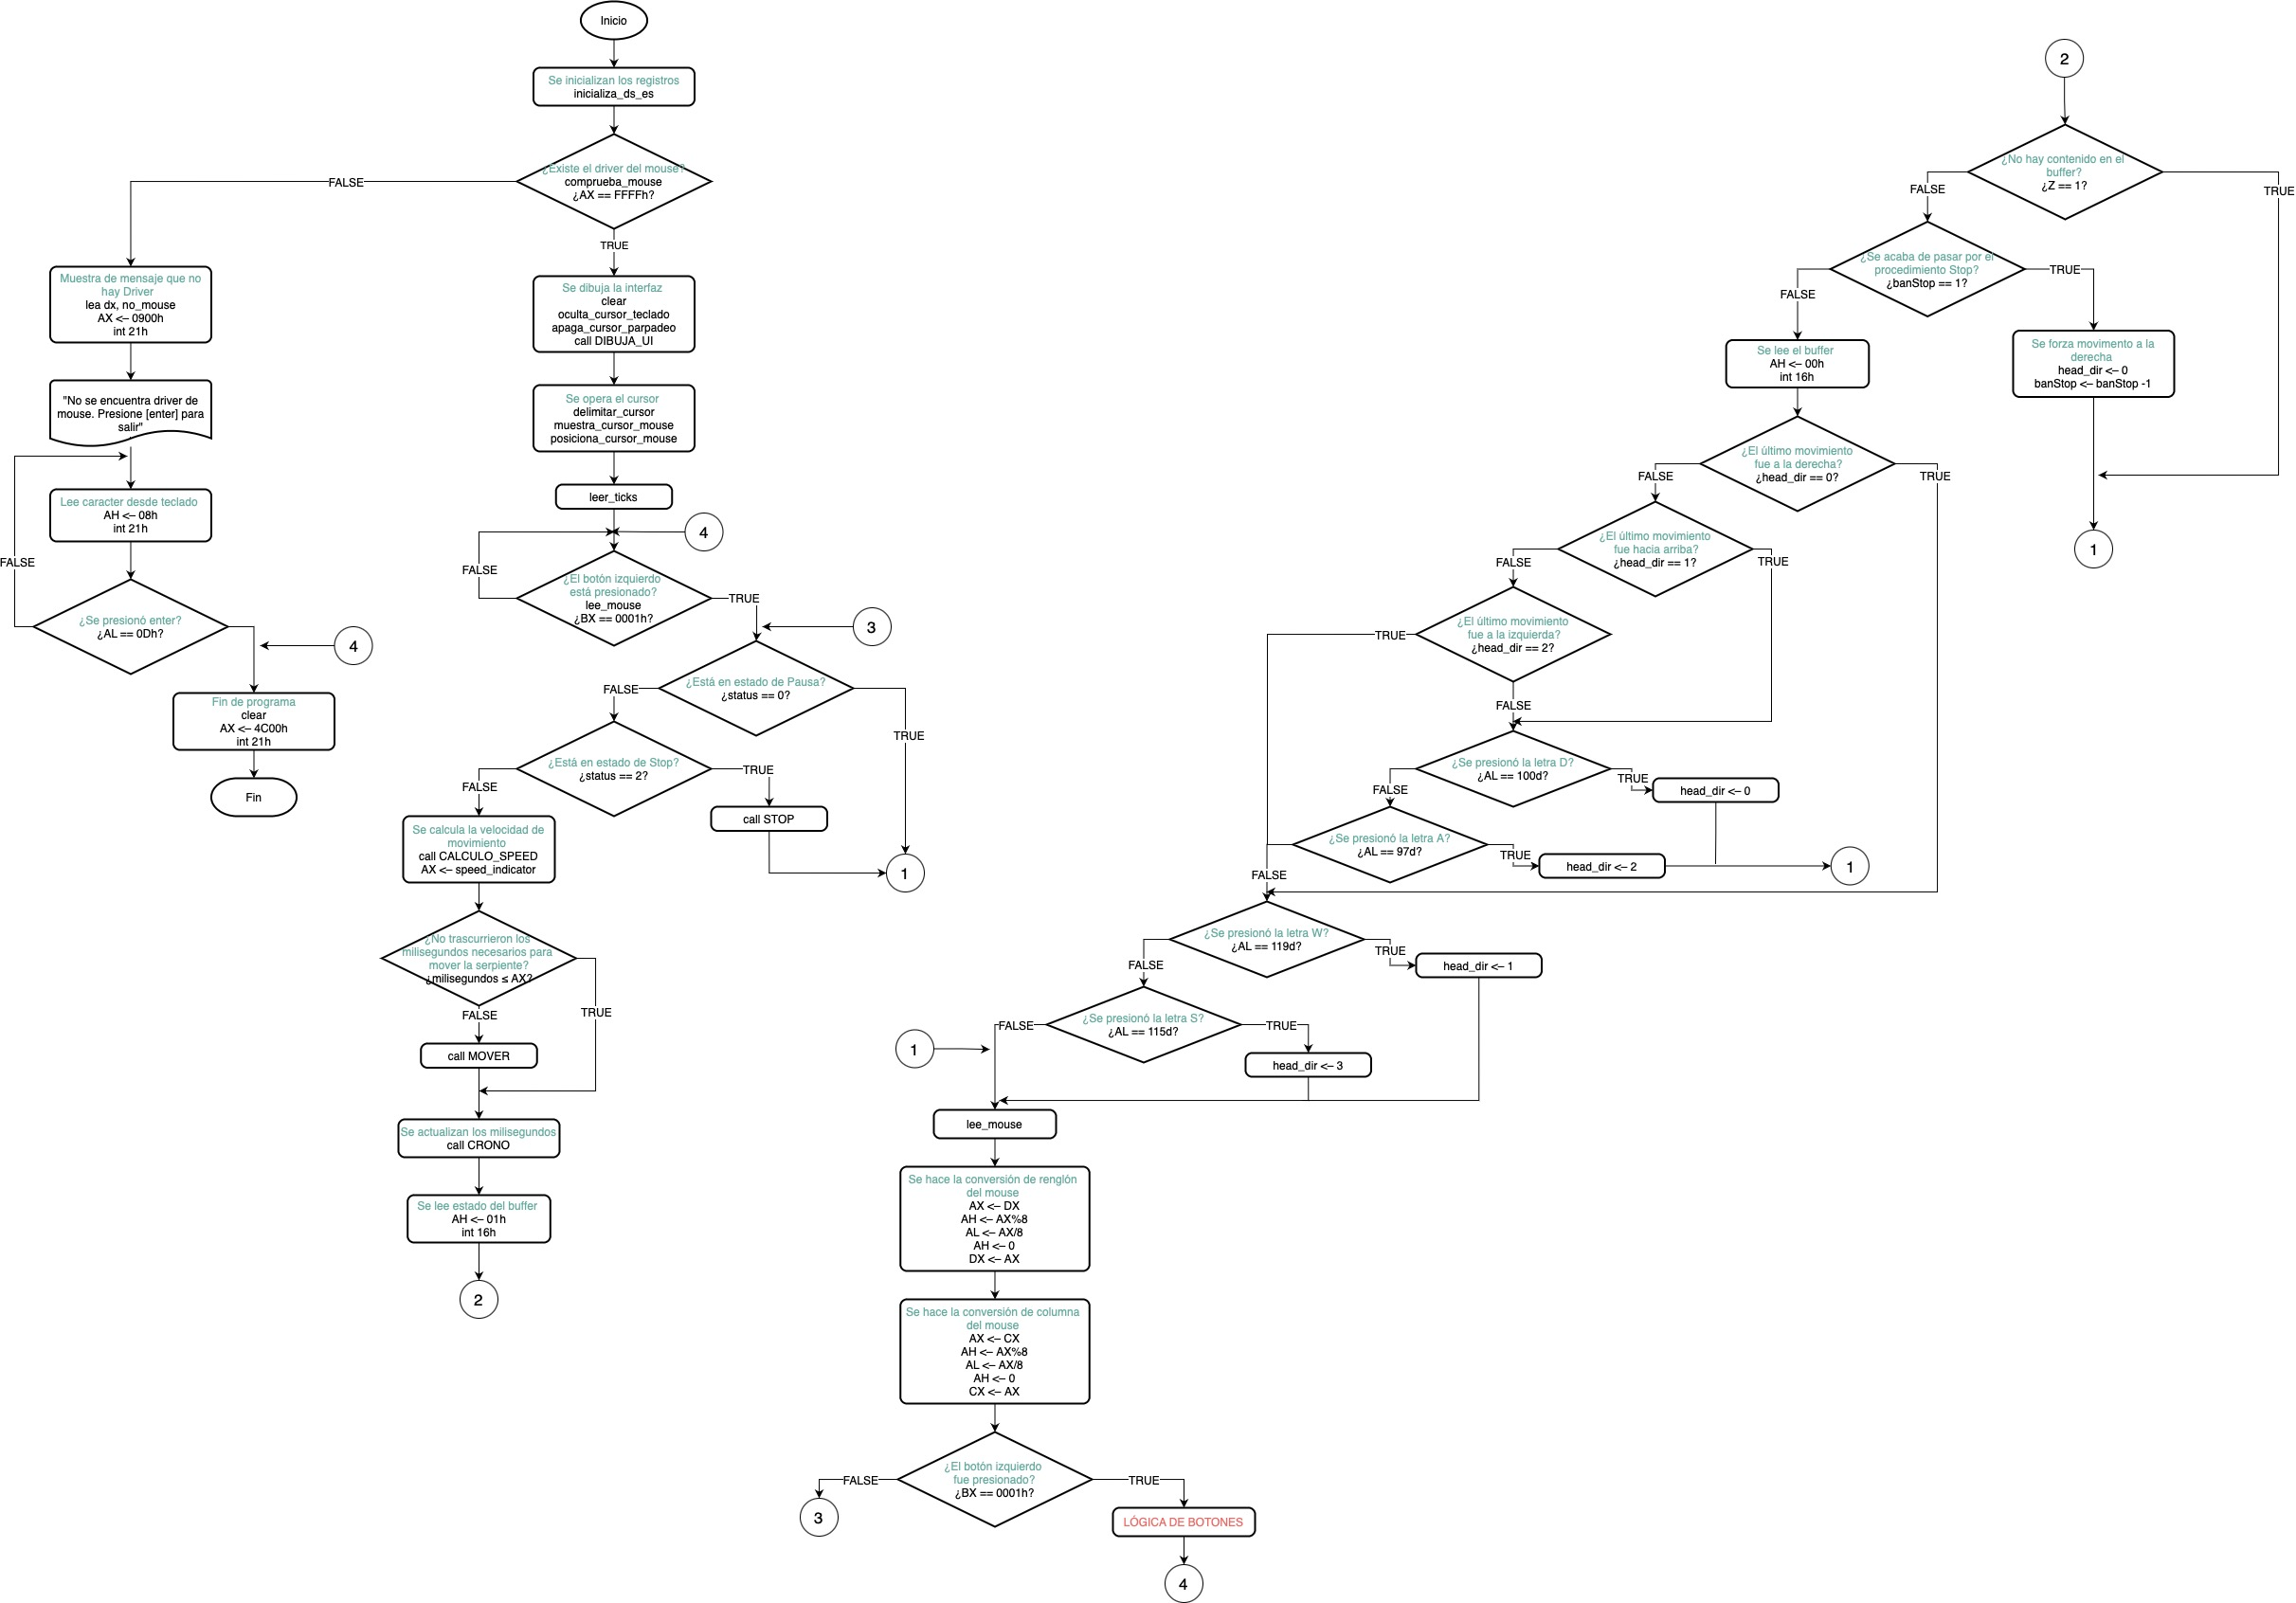
\includegraphics[height = 10cm]{img/diagramas/01DiagramaMain.jpg}
    \caption{Diagrama del flujo principal.}
    \label{fig:main}
\end{figure}

\subsubsection*{Procedimiento para mover}
El Diagrama \ref{fig:mover} describe el procedimiento para que la serpiente se mueva. Para este procedimiento se realiza una prueba de escritorio para que la serpiente se mueve uno hacia la derecha. Los datos iniciales son: tail = [30, 7],[30, 6],[30, 5], 0, $\dots$, head\_col = 30, head\_ren = 8, head\_dir = 0. Lo primero que se hace es borrar a las posiciones actuales con el procedimiento BORRA\_PLAYER. Después se guarda el valor de la cabeza actual en la pila por lo que el tope de la pila quedaría con los valores de [30, 8]. En la primera toma de decisión se compara head\_dir con 0 y se pasa la rama de verdadero. Por lo tanto, se le suma uno a la columna de la cabeza que queda como head\_col = 31. Se compara este nuevo valor de la cabeza con el valor del objeto para ver si fue comido. Esto se realiza con el procedimiento COMER\_OBJ y es lo último antes de mover los valores del cuerpo.

Para el cuerpo se realiza un \textit{loop} donde se recorren los valores del cuerpo. En el diagrama se muestra este proceso con i cuando en el programa se realiza con un apuntador a la dirección de memoria. En cuanto a lógica los procesos que se hacen son equivalentes. Se inicializa a i = 0 porque esa es la primera posición y a CX con el valor de la primera posición, CX = [30, 7]. 

Primera iteración: [30, 6] != 0, AX = [30, 6], tail = [30, 7],[30, 7],[30, 5], 0, $\dots$, CX = [30, 6], i = 2.

Segunda iteración: [30, 5] != 0, AX = [30, 5], tail = [30, 7],[30, 7],[30, 6], 0, $\dots$, CX = [30, 5], i = 4.

Tercera iteración: 0 == 0. Fin de las iteraciones.

Por último, se saca el valor del tope de la pila AX = [30, 8] y se le asigna al primer valor de tail, tail = [30, 8],[30, 7],[30, 6], 0, $\dots$. Con esto ya se recorrieron los valores que se tenían de la cola y la cabeza se movió en la dirección deseada. Se llama al procedimiento para verificar que no se haya comido el marco y se imprime la nueva serpiente. Los valores finales quedarían como: tail = [30, 8],[30, 7],[30, 6], 0, $\dots$, head\_col = 31, head\_ren = 8, head\_dir = 0. 

\begin{figure}
    \centering
    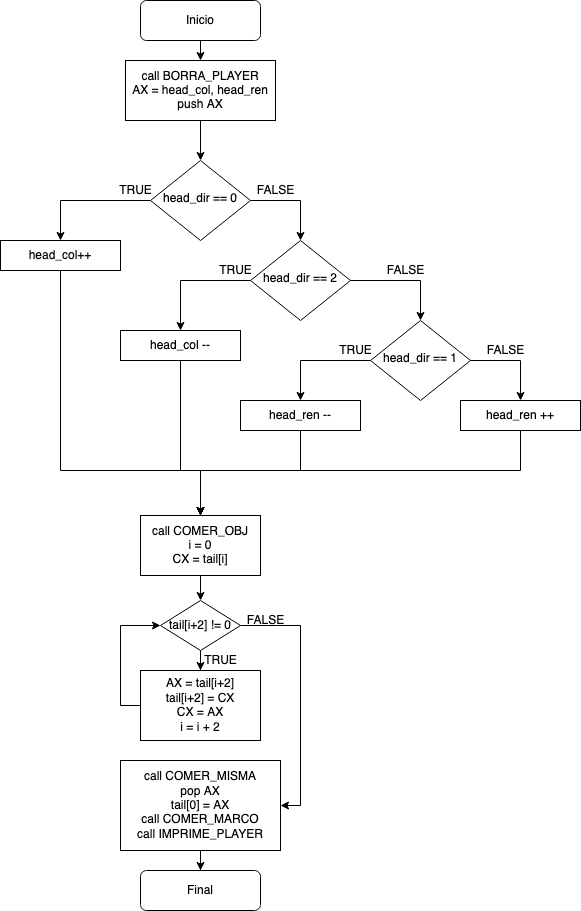
\includegraphics[height= 10cm]{img/diagramas/02DiagramaMover.png}
    \caption{Diagrama sobre el procedimiento para mover.}
    \label{fig:mover}
\end{figure}

\subsubsection*{Procedimiento para el marco}
Este procedimiento se manda a llamar en el procedimiento anterior y sirve para verificar que la serpiente no se haya comido el marco todavía y el usuario no haya perdido. Este proceso se encuentra representado en el Diagrama \ref{fig:marco}. Para la prueba de escritorio de este procedimiento se asumirá que el usuario se comió el marco inferior con los valores iniciales de head\_col = 42, head\_ren = 24. Primero se realiza la comparación de 24 == 0 con resultado falso, por lo que se pasa la siguiente comparación 24 == 24 con resultado verdadero. Se modifica el valor de la cabeza para evitar que la cabeza de la serpiente tenga la misma posición que un marco y se lo coma. En este caso se decrementa su valor en uno, head\_ren = 23. Se manda a llamar a STOP para que el juego se reinicie porque si se modifica la cabeza significa que el usuario se ha comido un marco y ha perdido. Si ninguno de los valores de la cabeza coincide con alguno de los marcos STOP nunca se manda a llamar y este procedimiento no modifica nada.

\begin{figure}
    \centering
    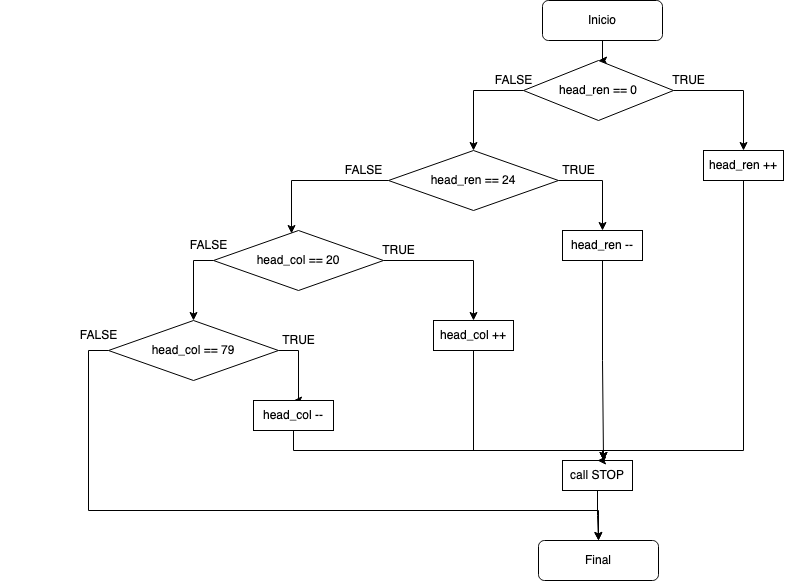
\includegraphics[height = 10cm]{img/diagramas/03DiagramaMarco.png}
    \caption{Diagrama para que no se coma el marco.}
    \label{fig:marco}
\end{figure}

\subsubsection*{Comer un objeto}
En el diagrama \ref{fig:comer} se puede observar el funcionamiento de manera gráfica del procedimiento que se encarga de ver si la serpiente se comió al objeto. Se tiene una condicional principal que compara la posición del objeto, dada por AX, con el valor de la cabeza, dada por BX. En caso de que sean iguales se inicia el proceso en donde se imprime al objeto de nuevo utilizando 2 procedimientos que ya se han explicado anteriormente. Después se puede ver que hay una comparación entre el valor del puntaje con el puntaje más alto. En caso de que es segundo sea menor, se copia el valor y se imprimen en pantalla. 

Para demostrar como funciona este procedimiento se realizará una prueba de escritorio. Empezamos con la posición original de la cabeza: [25, 12]; por lo que los valores de head\_col = 25, head\_ren = 12. El objeto se pondrá en una posición aleatoria (para que la prueba no sea tan larga se tomará un valor cercano a la cabeza). El objeto estará en [27, 2]; por lo que los valores de item\_col = 27, item\_ren = 15. En el momento en el que empiece el juego se moverá la serpiente a la derecha, entonces el valor de head\_col aumentará en 1: 25, 26, 27. En cada uno de esos momentos se va a actualizar el valor de AX: (190Ch, 1A0Ch, 1B0Ch), cada vez que se actualiza ese valor se va a hacer una comparación con el registro BX que tiene un valor de 1B0Fh. Como en ninguna de las 3 actualizaciones los valores son iguales, entonces no se realiza ninguna instrucción y continúa la ejecución del procedimiento que mueve a la serpiente. Considerando que el usuario direccionó a la serpiente de la manera eficiente, ahora la serpiente se moverá hacia abajo. Por lo que los valores de AX van a cambiar de la siguiente manera: 1B0Dh, 1B0Eh, 1B0Fh; este último valor en igual a BX, por lo que se entra en la opción verdadera de la condicional principal. Aquí se llama al procedimiento CALCULO\_ITEM. Los valores del objeto cambian a un valor aleatorio: item\_col = ??, item\_ren = ??. Como se utilizaron los valores iniciales: tail\_conta = 4, speed = 0, score = 0, hi\_score = 0. Después AX = 0004h, AX*2 = 0008h; SI = AX, SI = 0008h; [tail+8] = 1d; tail\_conta = 5 (aquí se aumenta el tamaño de la serpiente y se imprime un nuevo bloque). La velocidad se aumenta en 2: speed++, speed++: speed = 2. Se aumenta el score en 10 por lo que score = 10. Se hace la comparación entre score y hi\_score: ¿10 \> 0? Es verdad, por lo que hi\_score = score (hi\_score = 10). Y se acaba el procedimiento. La comparación de la cabeza y el objeto se va a hacer cada vez que se mueva la serpiente. 

\begin{figure}
    \centering
    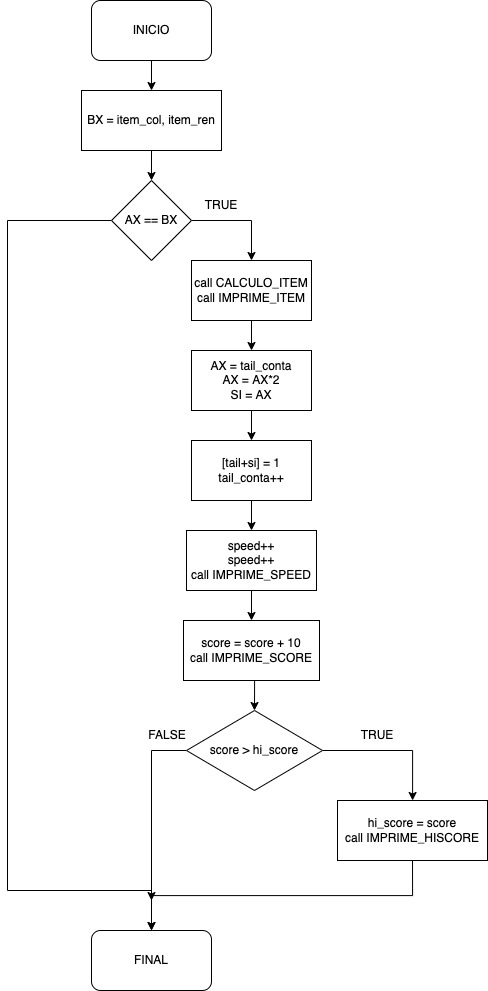
\includegraphics[height= 10cm]{img/diagramas/04DiagramaComerObjeto.jpg}
    \caption{Diagrama cuando se come un objeto.}
    \label{fig:comer}
\end{figure}

\subsubsection*{Lógica de Botones}
Con el Diagrama \ref{fig:botones} se representa la forma en que funcionan los botones que se tienen en el juego. Los botones pueden estar en tres secciones de renglones: en el renglón 0, del renglón 11 al 13 y del renglón 19 al 21. El primero se trata del botón para salir, el segundo de los botones para subir y bajar la velocidad y el tercero de los botones para cambiar el estado del juego. Se hará una prueba de escritorio para cambiar el estado, sobre los demás botones la prueba sería muy similar.

En la prueba de escritorio para cambiar el estado del juego se tiene que se intenta cambiar el estado a pausa (0). Se lee el mouse y sus valores son lee\_mouse = 20, 3. Se compara 20 == 0 con resultado falso, se compara 20 con 11, 12 o 13 todos siendo falsos y por último, se compara 20 con 19, 20 o 21 siendo verdadero. Se inician las comparaciones de las columnas para saber si se está pulsando el área de algún botón. En este caso, la primera toma de decisión se tiene que es cierta y el status cambia, status = 0. Por último, se hace un salto a mouse\_no\_clic para seguir con el flujo del programa de la serpiente. En la lógica de botones se utilizan los valores leídos por el mouse para decidir si se debe hacer alguna operación y en caso de que sí, cuál operación debe ser.

\begin{figure}
    \centering
    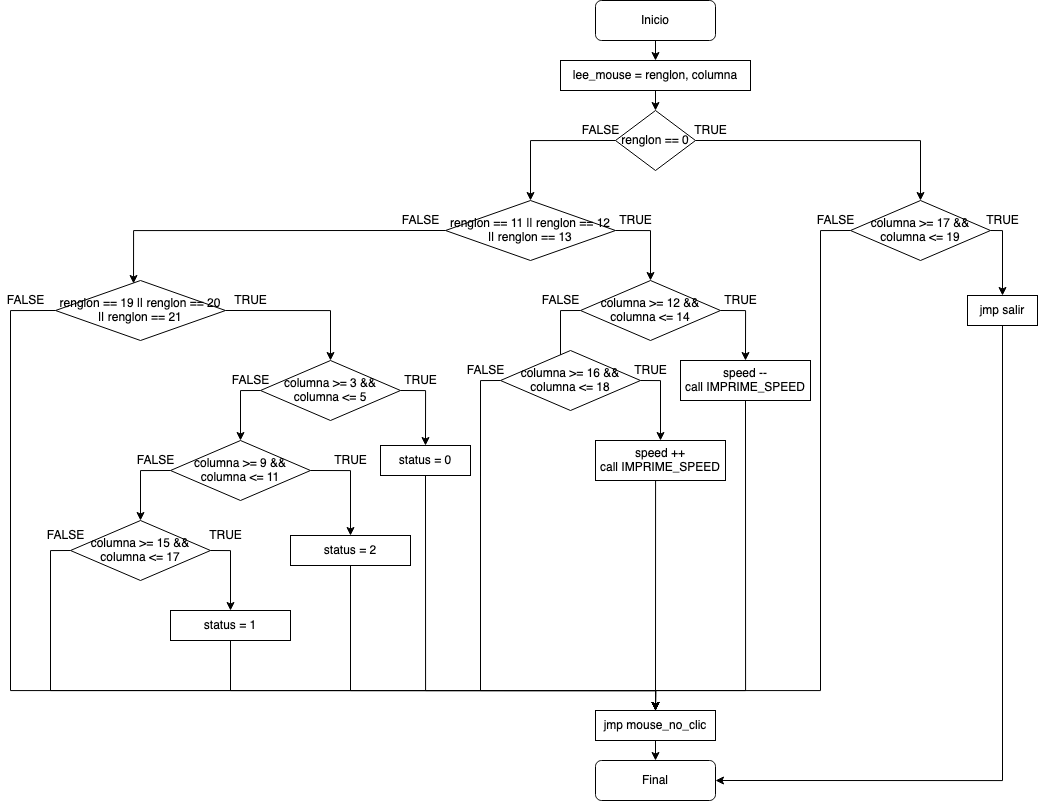
\includegraphics[height= 10cm]{img/diagramas/05DiagramaBotones.png}
    \caption{Diagrama sobre la lógica de botones.}
    \label{fig:botones}
\end{figure}

\subsubsection*{Procedimiento de reinicio y restablecimiento de datos iniciales}
En el diagrama \ref{fig:stop} se puede ver los 2 diagramas que se utilizan para cuando el usuario pierde una partida. Cualquiera que sea la razón (comerse a sí misma, pegarle a un marco o reiniciar el juego), estos 2 procedimientos entran en ejecución. Se puede apreciar el funcionamiento real del procedimiento en la siguiente prueba. 

Lo primero que sucede es que se iguala a conta con 4 (conta = 4). Se llama al procedimiento que borra al jugador en pantalla. Se utiliza la opción 0000h de la interrupción 1Ah. Después la variable flash se iguala al valor de DX, que es donde está la parte baja de los ticks: flash = 5F72h. Se le resta uno a la variable conta (conta = 3). Se produce un salto en el código que nos lleva a la sección donde se espera. Se vuelve a utilizar la interrupción con opción 1Ah. DX = 5F74h (nuevos ticks). Se restan ambos y ese es el nuevo valor de DX: DX = Dx - flash = 0002h. Se compara ese valor con 5d. Es menor, por lo que se salta de nuevo a esperar. Se vuelve a tomar un calor de los ticks. DX = 5F90h. Se hace la misma operación: DX = Dx - flash = 001Dh. Este se compara con 5, como es mayor se compara el contador con 0. En este caso es más grande ya que el contador es 3. Después se mueve el contador a AL: AL = 3. Después se divide entre 2. AL = 1, AH = ?. Se compara el residuo de la división que está guardado en AH con 0, viendo si el número es par. En este caso no es par, por lo que se salta a la sección aparece. Aquí se llama al procedimiento que imprime a la serpiente. Se usa la misma interrupción para tomar los ticks y se actualiza el valor de flash. DX = 6000h, flash = dx, flash = 6000h. Y decrece conta = 2. Se vuelve a entrar a "esperar" y se utiliza la interrupción para tener de nuevo los ticks. DX = 6010h, se restan flash y dx: DX - flash = 0010h. Este valor se compara con 5d. 10h es mayor que 5d, por lo que se compara el contador con 0. Como no son iguales se mueve el contador a al. AL = 2. Este valor se divide con 2. AL = 1, AH = 0. Se compara AH con 0, como son iguales, se salta a la sección "desaparece". De nuevo, se borra al jugador por el procedimiento para lo mismo, AX = 0000h, y se tiene la interrupción 1Ah. Se obtienen los ticks y se pasan a la variable flash: DX = flash = 6020h. Conta se reduce: conta = 1. Se salta a "esperar". Se vuelven a obtener los ticks. DX = 602Ch. Se restan DX = DX - flash = 000Ch. 0Ch es mayor a 5d, por lo que se compara conta con 0. Como no son iguales, AL = 1, AL/2: AL = 0, AH = 5. Como AH no es igual a 0, se pasa a la sección "aparece". Aquí se vuelve a utilizar la opción 0000h con la interrupción 1Ah. DX = flash = 603Ah. Y conta se hace 0. DX = 6045h. Se resta DX - Flash = 000Bh. Bh es mayor que 5d. Como el contador es igual a 0 se salta a la sección "después". Aquí se llama a una serie de procedimientos: BORRA\_PLAYER, REGRESA\_DATOSIN, IMPRIME\_PLAYER, IMPRIME\_SCORE, IMPRIME\_SPEED, BORRA\_ITEM, CALCULO\_ITEM, IMPRIME\_ITEM. La variable banStop se aumenta banStop = 1. La bandera de Speed que permite modificar la velocidad en el reinicio se actualiza con 1 y se acaba el procedimiento. 
Lo que pasa en el procedimiento REGRESA\_DATOSIN es que todos los valores de todas las variables que se usan en la ejecución del juego se ponen en su valor inicial. Eso incluye a la cabeza, a la cola y al cuerpo. 

\begin{figure}
    \centering
    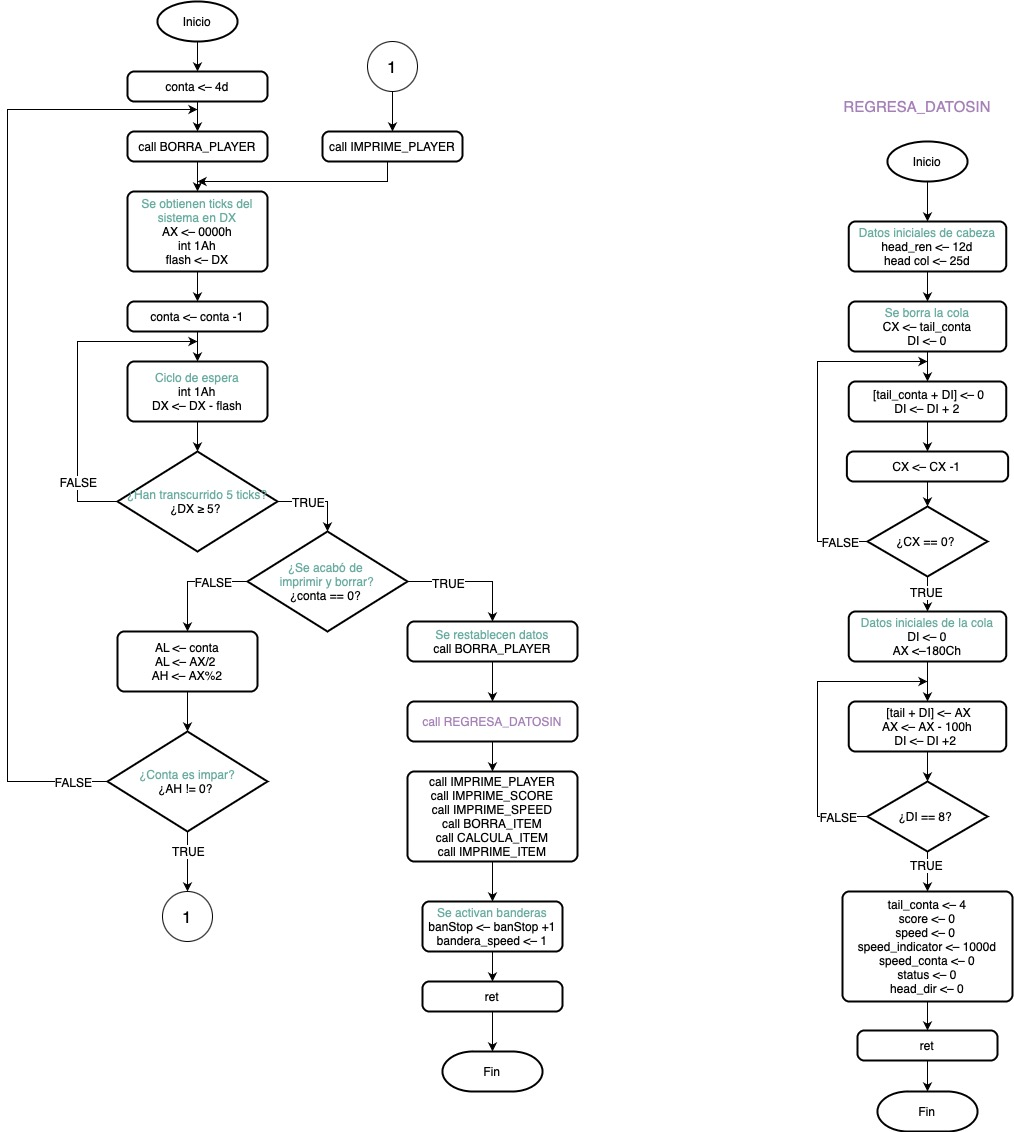
\includegraphics[height= 10cm]{img/diagramas/06DiagramaStop.jpg}
    \caption{Diagrama sobre el procedimiento reinicio y restablecimiento de datos iniciales}
    \label{fig:stop}
\end{figure}

\subsubsection*{Procedimiento para que no se coma a sí misma}
 En este diagrama \ref{fig:auto} se puede observar el comportamiento del procedimiento que se utiliza para estar seguros de que la serpiente no se pueda comer a ella misma. En este procedimiento se obtiene el valor de la cola. Se hace a BX un apuntador para la variable tail. Se toman los valores iniciales de la cabeza (éstos valores cambian pero para fines de la prueba se utilizará el inicial), head\_col = 25, head\_ren = 12. AX = 1100000001100b se compara AH con el valor de la cabeza. Como no son iguales, 25 != 24, se salta al valor siguiente de la cola. Aquí se le suma 2 a BX, se usa como apuntador y se compara con el valor de 0, al no ser iguales se regresa al loop. Tomemos el caso de que la siguiente parte del cuerpo si coincide con la cabeza. AH = 25, si se cumple esta condicional, se compara el renglón. AL = 12. Se cumple, de esta manera sabemos que la cabeza tiene una posición de [25, 12], y también se sabe que la segunda parte del cuerpo tiene posición [25,12]. Al ser así el status cambia a 2. Lo que producirá que el juego se detenga y se llame al procedimiento STOP.   
 
\begin{figure}
    \centering
    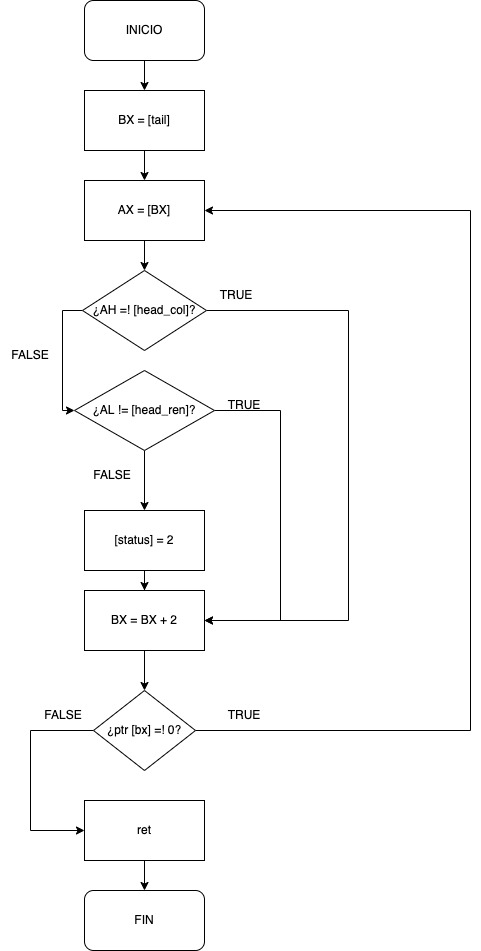
\includegraphics[height= 10cm]{img/diagramas/07DiagramaAutoComer.jpg}
    \caption{Diagrama sobre el procedimiento para que no se coma a sí misma}
    \label{fig:auto}
\end{figure}

\section*{Conclusión}
\subsection*{Barreiro Valdez Alejandro}
En este proyecto se pusieron en práctica todos los conceptos vistos sobre el lenguaje ensamblador vistos a lo largo del curso, y se investigaron nuevos conceptos para generar una versión del juego \textit{Snake} en lenguaje ensamblador. Fue un gran ejercicio como programador ya que es un proyecto muy robusto que necesita muchos conceptos, conocimientos técnicos e investigación por parte del desarrollador. Desarrollar este proyecto sirvió como muy buena práctica para reforzar todos los conceptos que se vieron a lo largo del curso y aprender sobre otros. Se cumplieron los objetivos y se resolvieron todos los problemas iniciales para poder generar un juego totalmente funcional. Se codificaron las diversas especificaciones que se requerían para que funcionara el juego y con cada una de las soluciones para los sub-problemas se logró el objetivo mayor de codificar el juego. Primero, se tuvo que entender el código base y entender qué se podía cambiar de él para utilizarlo y qué se podía reusar. A partir de esto, los integrantes del equipo diseñaron diferentes soluciones a los diferentes requerimientos que se tenían para hacer el juego funcional. Se generaron procedimientos que en su momento parecían muy complicados como el de mover la serpiente, generar un objeto aleatorio en la pantalla y leer el mouse. Todo esto se logró a través de investigación y colaboración de los participantes y gracias a ello se pudieron resolver los diferentes problemas que planteaban codificar cada uno de los requerimientos en lenguaje ensamblador. Con este proyecto, no solo se logró codificar un juego funcional de Snake, también se reforzaron y ampliaron los diferentes conocimientos que se tenían sobre el lenguaje ensamblador. Este código involucra la manipulación de registros, operaciones aritméticas y lógicas, control de flujo en lenguaje ensamblador, uso de macros y procedimientos, lectura de mouse, impresión a pantalla de una interfaz gráfica y lectura de teclado, entre muchos otros temas. Se pude concluir que los problemas planteados fueron resueltos y se cumplieron los objetivos de este proyecto.

Este proyecto me permitió aprender muchas habilidades valiosas para el programador, no solo en el aspecto técnico, también en el aspecto colaborativo. Se reforzaron temas sobre el lenguaje ensamblador que se vieron a lo largo del curso. Lo primero que se reforzó fue la interpretación y lectura del código al entender el código base que proporcionó el profesor. También se reforzaron los diferentes conceptos sobre la codificación en lenguaje ensamblador. Se realizaron operaciones aritméticas y lógicas a lo largo de todo el código y se manipularon variables y registros para manejar la información del programa. Se utilizaron salto condicionales a lo largo de todo el código para controlar el flujo del programa y tomar diferentes decisiones. Gracias a este control de flujo se logró generar aspectos como el movimiento o la reacción ante alguna tecla o un click del teclado. Además de reforzar concepctos de lenguaje ensamblador se aprendieron algunos nuevos como el modo vídeo y la manera en que se imprimió la interfaz de usuario. Otros conceptos útiles los cuales se vieron con el proyecto fue la lectura de datos del teclado y la lectura de los datos del mouse. Estos conceptos son altamente útiles para cualquier lenguaje de programación y le dan un dinamismo adicional al juego. Otro concepto esencial que fue de gran utilidad fue el manejo del tiempo que transcurre en un programa. Este nuevo concepto que se aprendió para el juego sirvió para que el juego se pueda desarrollar a través del tiempo. Por último, se desarrollaron nuevas técnicas colaborativas que no se habían utilizado en proyectos anteriores de programación. Se trabajó con herramientas que permiten el trabajo y la comunicación a la distancia. Se utilizaron plataformas como GitHub y Overleaf para generar el código y el reporte del proyecto de manera colaborativa. Gracias a estas plataformas se logró una colaboración fácil de integrar y un trabajo donde todos los integrantes aportaron. Este proyecto proporcionó diferentes conocimientos útiles para mis habilidades como programador. Sirvió para repasar y aprender conceptos sobre la programación en lenguaje ensamblador y colaborar con otros programadores para generar un proyecto funcional.

En este proyecto se pudieron visualizar las ventajas y desventajas que se tienen en la programación en lenguaje ensamblador. En cualquier otro lenguaje de programación de alto nivel programar este juego tendría menos líneas de código y probablemente el código sería más entendible. Los lenguajes de programación de alto nivel contienen muchas sentencias que permiten ahorrar código, pero muchas veces no se sabe a bajo nivel qué hace cada una de estas sentencias. El código generado en el proyecto no es muy entendible para personas que no sepan sobre lenguaje ensamblador y puede parecer muy complejo todo lo codificado. Sin embargo, esto permite mucha libertad al programador de generar procesos que en otro lenguaje no se pueden hacer. Se controla toda la memoria que es utilizada y se tiene mucha eficiencia sobre las operaciones que se hacen y la memoria que se utiliza. Otra ventaja es que aunque en este proceso se realizan demasiadas operaciones en un lapso de 3 milisegundos, la eficiencia que ofrece el lenguaje ensamblador permite que esto se pueda realizar y no se ven problemas cuando se llegan a estas velocidad. En otros lenguajes de programación, probablemente se podrían observar problemas a la hora de ejecutar un código que realiza tantas operaciones en muy poco lapso de tiempo. Con este proyecto se observó cuáles son algunas de las ventajas y desventajas del lenguaje ensamblador; y se observó la eficiencia que tiene un programa en lenguaje ensamblador. Sin duda, esto fue un gran proyecto que me permitió mejorar mis habilidades como programador y mejorar mis conocimientos sobre el lenguaje ensamblador.

\subsection*{Piña Félix Emilio}
El objetivo de este proyecto era la codificación de un juego de "Snake" en lenguaje ensamblador. Se proporcionó una base de código sobre la cuál se tenía que desarrollar todas las funcionalidades del juego. Uno de los retos más complicados del proyecto fue el trabajo en equipo, debido a la distancia y a la imposibilidad del trabajo en persona, se requirió utilizar herramientas como Github, Overleaf, entre otras. El proyecto requirió bastante información que, por suerte, fue proporcionada por el profesor. Este proyecto puso a prueba todo lo que se aprendió en el año. Las operaciones de control de flujo fueron de vital importancia para la resolución del problema. A falta de una operación condicional usual como las que se encuentra en los lenguajes de alto nivel, el trabajo que se tenía que poner para realizar la comparación resultaba tedioso. Sin embargo, existieron muchas ventajas de usar el lenguaje ensamblador. Este tipo de ventajas se racionalizaron después del análisis del código final. El programa tiene que hacer una cantidad importante de comparaciones, cada vez que la serpiente se mueve. Si el lenguaje de programación tuviera un mal tiempo de ejecución, el juego sería muy difícil de ejecutar. Al ser el tipo de programación más rápida con el que se ha programado hasta ahora, es necesario alabar la velocidad con la que se ejecutan 1175 líneas de código. Hubo aspectos del proyecto que presentaron una complejidad más alta que otros, por ejemplo: la lectura de las flechas del teclado en tiempo de ejecución fue un trabajo que llevó más tiempo que la codificación del comportamiento del juego cuando se toca un marco. 

El lenguaje ensamblador presenta dificultades que son intrínsecas a la codificación base del lenguaje. Al estar más cerca del lenguaje máquina, es más complicado expresar lo que queremos hacer. Este nivel menor de abstracción trajo consigo un mayor esfuerzo mental, ya que no se parece mucho a lo que estamos acostumbrados a pensar o a programar. Sin embargo, gracias a las clases que se impartieron en este semestre, así como la práctica que se adquirió durante la realización ejercicios, tareas y exámenes, se presentó una ligera afinidad al lenguaje ensamblador. Mientras que el proyecto no careció de dificultad, es de mi entendimiento que ninguno de mis compañeros de equipo sufrió frustración al no poder expresar la solución teórica de los problemas nos tocó enfrentar de manera práctica. Gracias a una buena documentación que se llevó a cabo durante toda la codificación del proyecto, era sencillo ponerse al corriente de los cambios que se habían hecho al proyecto. 
El trabajo de documentación fue de gran ayuda para comprender de manera profunda la manera en la que se resolvieron los problemas. Las pruebas de escritorio, los diagramas de flujo y las justificaciones de las soluciones codificadas sirvieron para nosotros mismos entender aún más lo que habíamos hecho. El uso de procedimientos, como se puede notar después de leer este documento, fueron una de las bases más importantes durante la resolución del problema. También se pudo notar que en cada procedimiento se utilizaban otros diferentes para poder lograr la ejecución exitosa. Por ejemplo, se codificó el movimiento de la serpiente primero, después se codifico el cálculo y la impresión del objeto. Un aspecto que me llamó la atención del proyecto fue la sencillez inesperada de la codificación de la interfaz gráfica. Cuando se propuso el proyecto, no tenía idea de como hacer para que se pudiera ver el juego en la pantalla. Una vez vistos los vídeos y analizado el código, fue grato encontrar que no era tan complicado. Las bases que tenemos en el lenguaje ensamblador eran más que suficientes para poder enfrentar este problema de manera exitosa. Al final se utilizaron los 3 procedimientos para poder codificar lo que pasaba cuando la serpiente comía a un objeto. Esta manera de codificar requería de bastante comunicación entre los 3 autores de este código. Todos los procedimientos tuvieron que ser explicados a las partes que no la habían codificado, y de esa manera, que se pudiera construir un proyecto de la calidad del que se presentó en esta ocasión. Aunque ya se mencionó la dificultad de la programación de este proyecto a distancia, creo que nuestro equipo trabajó de manera extraordinaria. 

Este proyecto es uno del que estoy orgulloso. Se trabajó bastante en la codificación, así como en la documentación. Sin embargo, siento que el trabajo en equipo se llevó a cabo de manera extraordinaria. Se cumplieron todos los objetivos del proyecto. Éste nos dejó con un mayor entendimiento y conocimiento de lo que se puede hacer con el lenguaje ensamblador. También nos dejó con un grato recuerdo de lo que es posible cuando se trabaja en equipo. 

\subsection*{Zepeda Baeza Jessica}
El proyecto final del curso fue hacer un juego \textit{Snake} en lenguaje ensamblador. Para ello se nos proporcionó un código base que, al ejecutar, mostró la interfaz gráfica del juego así como algunos elementos indispensables como el puntaje, la velocidad y los botones a utilizar. Por otra parte también el código proporcionó un modelo con el que el juego iba funcionar. Es decir, se planteó la idea de jugar con clicks del usuario para continuar o detener el flujo del sistema y realizar los procesos necesarios. El código base además nos guió en cuanto a la organización del flujo para entender dónde colocar aquellas instrucciones que analizan los botones o las teclas. El código y el vídeo base fueron elementos esenciales para el proyecto por lo mencionado y además porque nos proporcionaron un razonamiento más orientado tanto a lenguaje ensamblador como a una lógica de hacer un juego interactivo. 

El trabajo en equipo fue una ventaja y una desventaja ya que al realizar código cada quien tiene una idea distinta y no hay una forma correcta de lograr un cierto objetivo. La distancia tampoco ayuda mucho ya que el código puede sufrir cambios pequeños e importantes a los que todos se deben de ir actualizando y tomando en cuenta. Empezar a realizar las funciones del juego y los distintos estados fue sencillo ya que el equipo tenía una idea clara de hacer suceder las cosas así como la manera de implementarlo en el flujo principal. Una gran ayuda fue el uso de Github que nos permitió llevar un proceso claro de las modificaciones del código. 

Por otra parte, la resolución de problemas fue muy clara y fluida ya que nos regimos con la idea de resolver el problema más grande cada vez. Es decir, lo primero fue hacer mover a la serpiente y calcular las velocidades a las que puede ir. Una vez que se mueve, lo siguiente fue hacer que comiera y creciera pero eso involucraba el calcular dónde acomodar aleatoriamente un objeto por lo que se resolvió eso primero. Otro ejemplo fue el procedimiento de reinicio el cual sucedía al comerse a si misma o chocar con un marco o presionar el botón \textit{Stop}. Lo que se realizó fue resolver el procedimiento de reinicio al presionar el botón ya que y se tenían la lógica de botones. De esa forma, se pudo utilizar al resolver el problema de “perder” y acomodar dichos procesos al procedimiento ya existente. En varias ocasiones fue notoria la aplicación de modularidad en el código.

Otro factor del que fuimos conscientes fue toda la documentación. Muchas veces se codifican tantos procesos que se pierde el programa en general. Pero eso no sucedió aquí gracias al documento escrito y los diagramas de flujo y pruebas de escritorio. Incluso partes que probablemente sólo un integrante del equipo realizó se entendieron a la perfección al tener que explicar con palabras y analizar lo que realmente pasaba en las líneas de código. Al acabar tanto el código como el documento nos dimos cuenta de que conocíamos el programa a la perfección. De la misma forma nos dimos cuenta de líneas de código que podrían evitarse o hacer más eficientes. Nos dimos cuenta de lo importante que es el análisis y qué hay cosas que al codificar no se ven y son importantes. 

Para concluir, considero que este proyecto me deja tres cosas a destacar. La primera tiene que ver con el manejo de lenguaje ensamblador, en un principio era complicado saber dónde poner saltos y como acomodar las líneas para tener menos de ellas y menos etiquetas. También hice un mejor manejo de procedimientos y de macros y comprendí en qué casos usar cuál. El segundo aprendizaje fue el razonamiento adecuado para un programa como este. Estaba acostumbrada a programas con ejercicios pequeños y al tener que programar un juego tuve que tomar en cuenta más cosas como el usuario y que se manejan más datos, más variables y se tienen que hacer procesos que se adecuen a las modificaciones que en un futuro se pueden realizar. El último aprendizaje es el manejo de código. Al no tener estructuras grandes para el control de flujo o manejo de datos, me di cuenta cuando son útiles y necesarios. Me di cuenta de lo que he aprendido en los últimos semestres y como lo aplico en un caso real. Me pareció un muy buen proyecto final y el hecho de ser en lenguaje ensamblador lo hizo más desafiante y con un nivel adecuado de dificultad.

\end{document}
